\documentclass[12pt]{article}

\usepackage[margin=1in]{geometry}
\usepackage{amsmath,amsthm,amssymb}
\usepackage{fancyhdr}
\usepackage[small,compact]{titlesec}
\usepackage{float}

\lhead{Erich Menge}
\chead{\classnameandsection}
\rhead{\homeworktitle}

\pagestyle{fancy}

\newcommand{\sethomeworknumber}[1]{
  \newcommand{\homeworktitle}{Homework #1}
}

\newcommand{\N}{\mathbb{N}}
\newcommand{\Z}{\mathbb{Z}}
\newcommand{\homeworkheader}[1]{
  \title{\vspace{2in}\homeworktitle}
  \author{Erich Menge (X.500: menge053, Student ID: 4624713) \\
  #1}
  \maketitle
  \newpage
}

\newenvironment{problem}[1]{
  \ignorespaces
  \section*{Problem #1}
}{
  \ignorespacesafterend
}

\newenvironment{solution}{
  \ignorespaces
  \subsection*{Solution}
}{
  \ignorespacesafterend
}

\newcommand{\classnameandsection}{CSCI 4011 Formal Languages And Automata Theory Section 3}

\usepackage{graphicx}
\usepackage{listings}

\sethomeworknumber{5}

\begin{document}

\homeworkheader{\classnameandsection}

\begin{problem}{21.3-1}
  Redo Exercise 21.2-2 using a disjoint-set forest with union by rank and path compression.
  \begin{solution}
    \begin{figure}[H]
      \centering
      \caption{Structure for disjoint-set forest with path compression after first set of unions}
      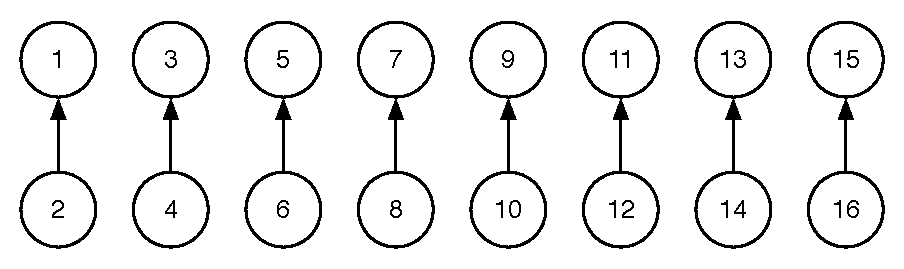
\includegraphics[scale=.5]{21_3_1_1.eps}
    \end{figure}
    \begin{figure}[H]
      \centering
      \caption{Structure for disjoint-set forest with path compression after second set of unions}
      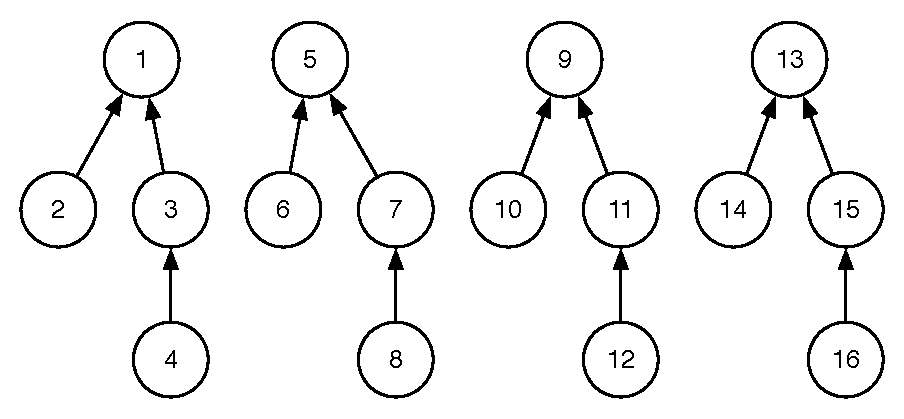
\includegraphics[scale=.5]{21_3_1_2.eps}
    \end{figure}
    \begin{figure}[H]
      \centering
      \caption{Structure for disjoint-set forest with path compression after final set of unions}
      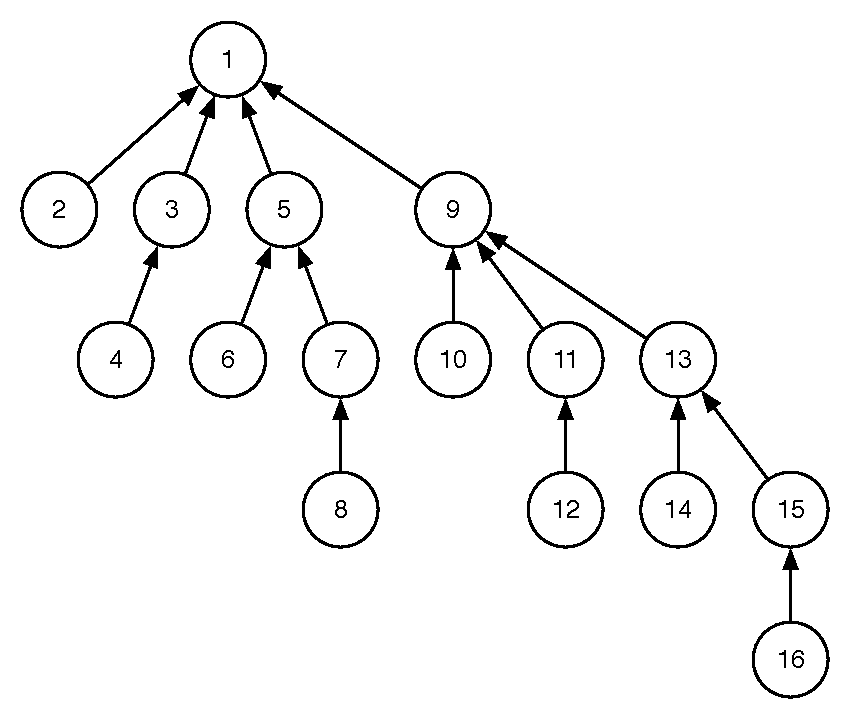
\includegraphics[scale=.5]{21_3_1_3.eps}
    \end{figure}
    \begin{figure}[H]
      \centering
      \caption{Structure for disjoint-set forest with path compression after find-set operations}
      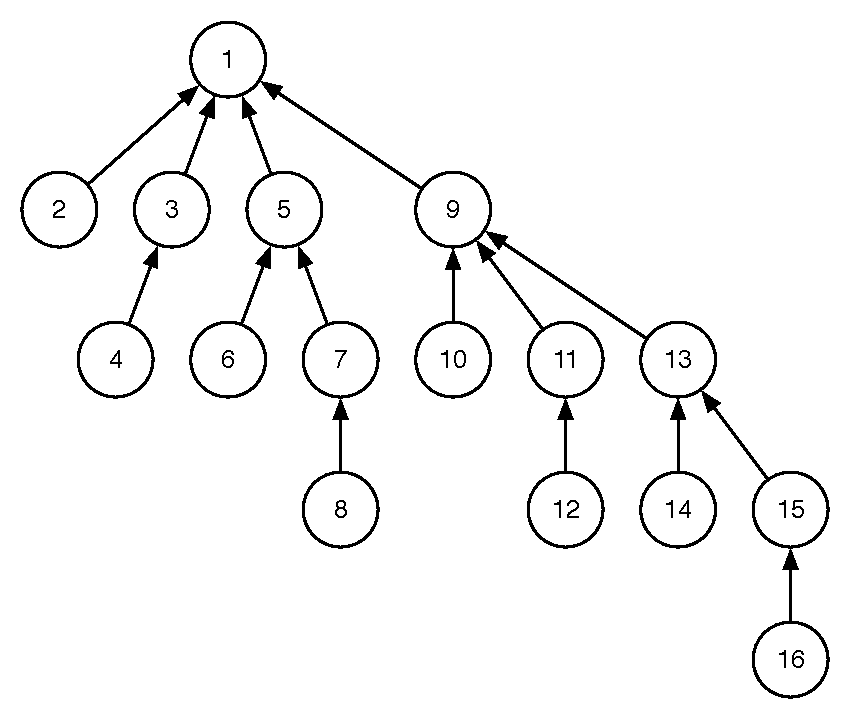
\includegraphics[scale=.5]{21_3_1_4.eps}
    \end{figure}
    Find-set(2) and Find-set(9) both return ``1''. In fact any find-set will return ``1'' now because it is the root of
    the tree.
  \end{solution}
\end{problem}

\begin{problem}{21.3-4}
  Suppose that we wish to add the operation PRINT-SET(x), which is given a node x and prints all the members of x's set,
  in any order. Show how we can add just a single attribute to each node in a disjoint-set forest so that PRINT-SET(x)
  takes time linear in the number of members of x's set and the asymptotic running times of the other operations are
  unchanged. Assume that we can print each member of the set in O(1) time.
\end{problem}

\begin{problem}{15.2-2}
  Give a recursive algorithm MATRIX-CHAIN-MULTIPLY(A,s,i,j) that actually performs the optimal matrix-chain
  multiplication, given the sequence of matrices $(A1, A2, \ldots, A_n)$, the $s$ table computed by MATRIX-CHAIN-ORDER, and
  the indices i and j. (The initial call would be MATRIX-CHAIN-MULTIPLY(A,s,1,n).)
  \begin{solution}
    \begin{lstlisting}
      matrix_chain_multiply(a[], s[], i, j)
        if i==j
          return a[i]
        else
          return matrix_multiply(
            matrix_chain_multiply(a, s, i, s[i][j]),
            matrix_chain_multiply(a, s, s[i][j] + 1, j)
          )
        end
    \end{lstlisting}
  \end{solution}
\end{problem}

\begin{problem}{15.2-4}
  Describe the subproblem graph for matrix-chain multiplication with an input chain of length $n$. How many vertices
  does it have? How many edges does it have, and which edges are they?
  \begin{solution}
    Each subproblem can be represented by a cell in a table $i\times j$. Where $j = i + l - 1$ and $l = 2\ldots n$ and
    $i = 1 \ldots (n - l + 1)$. Only half of the table is used though so we have $\frac{n(n - 1)}{2}$ verticies. Also
    we're looking for every combination of pairs, which can be represented as $\binom{n}{2} = \frac{n(n - 1)}{2}$.
    \br
    We want each subproblem to only be visited once and we accomplish this by storing the values in the table. As such
    we have $\frac{n(n - 1)}{2} - 1$ edges. Each edge is directional pointing to sub-problems and sub-problems pointing
    to sub-problems of theirs.
  \end{solution}
\end{problem}

\begin{problem}{15.3-2}
  Draw the recursion tree for the MERGE-SORT procedure from Section 2.3.1 on an array of 16 elements. Explain why
  memoization fails to speed up a good divide-and-conquer algorithm such as MERGE-SORT.
  \begin{solution}
    \begin{figure}[H]
      \centering
      \caption{Recursion map for merge-sort with 16 elements.}
      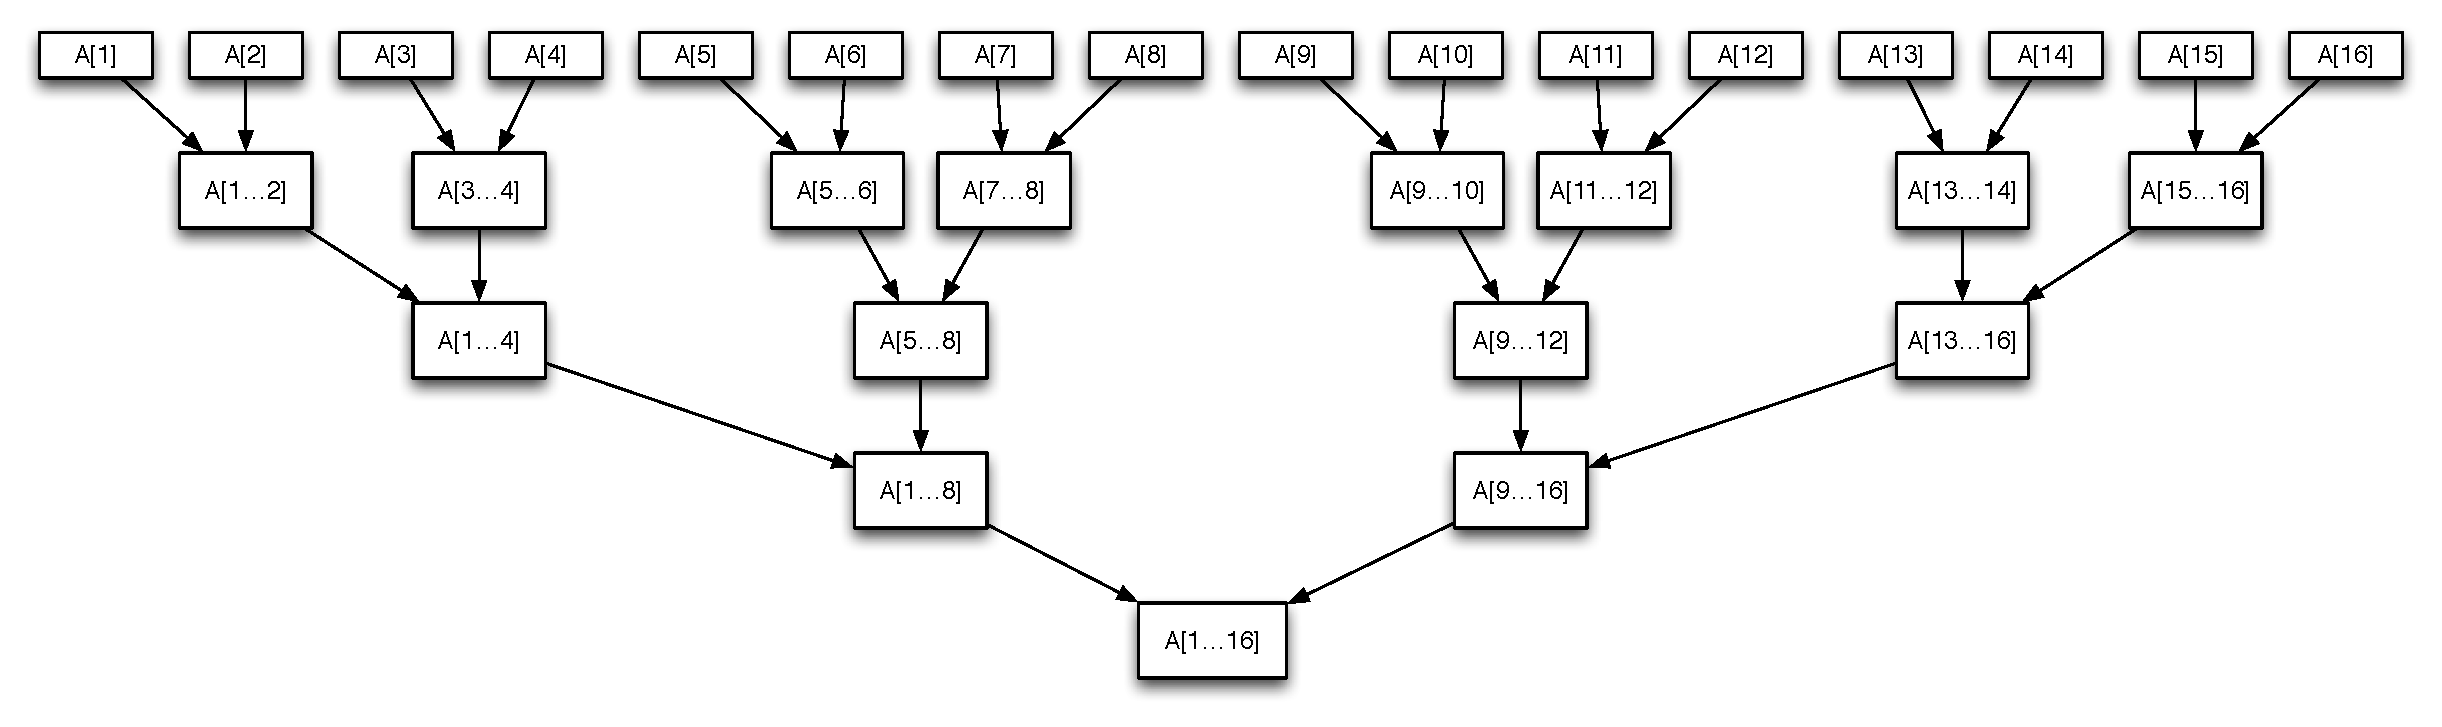
\includegraphics[scale=.35]{15_3_2.eps}
    \end{figure}
    Memoization is a technique used when recursive paths would otherwise be followed more than once. Merge-sort splits
    the array in half each level of recursion, and then each split is visited, and so on until the individual nodes are
    reached. Since each split needs to return before merge-sort returns (down to the individual nodes), each path is
    only visited once.
  \end{solution}
\end{problem}

\begin{problem}{15.3-3}
  Consider a variant of the matrix-chain multiplication problem in which the goal is to parenthesize the sequence of
  matrices so as to maximize, rather than minimize, the number of scalar multiplications. Does this problem exhibit
  optimal substructure?
  \begin{solution}
    Yes. This can be done the same way as the minimization. The matrices would still be grouped $(A_i \ldots A_k)(A_{k +
    1} \ldots A_j)$ only this time we would take $c_{i,j} = max(c_{i,k} + c_{k+1,j} + p_{i - 1}p_kp_j)$. Then the same
    tables as before could be created to store the maximum cost of each sub-problem. Therefore each sub problem is
    optimal.
  \end{solution}
\end{problem}

\end{document}
